\hyphenation{clCreateSubDevices}

%%%%%%%%%%%%%%%%%%%%%%%%%%%%%%%%%%%%%%%%%%%%%%%%%%%%%%%%%%%%%%%%%%%%%%%%%%%%%
\section{OpenCL and Device Fission} \label{sect:openCL}

OpenCL consists of an API for coordinating \textit{parallel computation across heterogeneous processors} (CPU, GPU and potentialy any other processor) and it is supported by a wide range of systems and platforms, making it the perfect choice for parallel computation not only on traditional desktop CPU-GPU configuration, but also on embedded systems.
OpenCL was initially developed by Apple, but is now maintained by the Khronos Group (http://www.khronos.org) that, in 2011, released the 1.2 version of the API, introducing new features such as enanched image support, built-in kernels and \textbf{device partitioning} (also known as Device Fission).\\
Since the strength of OpenCL is its heterogeneity, to compile and to execute and OpenCL application, one must install on the system the libraries specific to the target platform, and usually each hardware manufacturer provide its own SDK to develop and run OpenCL applications.

%-----------------------------------------------------------------------------
\subsection{OpenCL Architecture} \label{sect:openCLArch}

To define the structure of an OpenCL application, first we will introduce its core components. Some of these components (Host and Kernels) are ``software components'' that, together, form the core of an OpenCL executable, while other components (Compute Devices and Units) refer to the underlying hardware that has to run our application.\\
The architecture of an OpenCL application is summarized in \textbf{Figure \ref{fig:OpenCLArch}}, and the main components that needs further investigation are the \textbf{Host} (executed on the CPU), the \textbf{Kernels} (executed on the processig elements of the OpenCL device) and the \textbf{device}. We'll now introduce the concepts behind the host and the device; kernels and their implementation will be discussed later in Section \ref{sect:kernelImplementation} \\

\begin{figurehere}
 \centering
 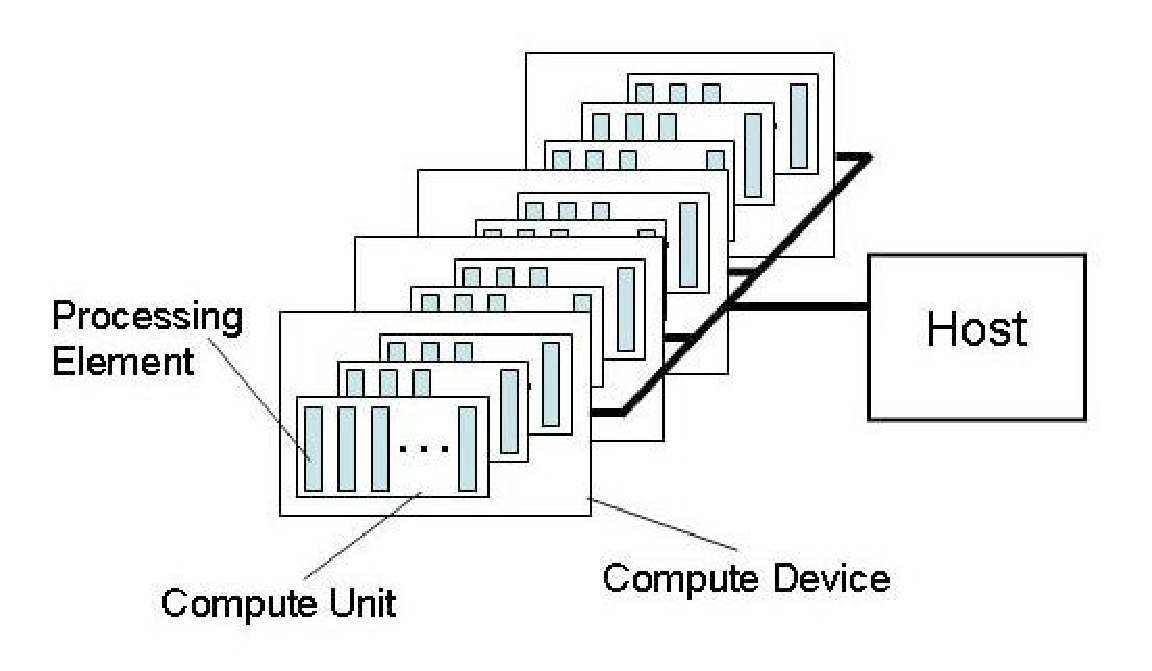
\includegraphics[width=8cm, height=4cm]{./eps/OpenCLArch.eps}
 \caption{OpenCL Architecture}
 \label{fig:OpenCLArch}
\end{figurehere}

\subsubsection{The Host}
The Host can be viewed as the \textbf{controller} of the application. It usually doesn't perform any task specific to the domain of the application and its main function is only to setup and configure the environment, to issue commands to the compute units and to coordinate the kernels. Since the host is basically a ``standard'' executable that executes ``normal'' code, \emph{it is always executed on the CPU and never on the GPU}.\\
Here's list of the main tasks that every host should do:

\begin{enumerate}
	\item Declare the necessary structures (Kernels, devices, memory objects...)
	\item Query for hardware capability (Number of devices available, number of processing units, buffers size...)
	\item Obtain and lock hardware resources
	\item Create and initialize memory objects (see Section \ref{sect:memory})
	\item Create kernels
	\item Issue orders to kernels (Launch, synchronization, memory management)
	\item Retrieve output data from kernels
	\item Manage errors
	\item Release of hardware resources, deallocate memory, and final cleanup.
\end{enumerate}

\begin{CLCode}
In OpenCL the host is a standard C/C++ application implemented inside the classical 'main' function. Every host must always implement and initialize these five data structures in order to properly setup an OpenCL environment:\\
\textbf{cl\_device\_id} to obtain an handle to the hardware device,\\
\textbf{cl\_kernel} to have a reference to each kernel implemented,\\
\textbf{cl\_program} to define the main program that contains all the kernels,\\
a \textbf{cl\_command\_queue} for each kernel, used to issue commands to them ,\\
a \textbf{cl\_context} that wraps all programs, kernels, devices and memory object of an OpenCL application.\\
In Appendix \ref{appendix:B} you can see an example of OpenCL host implementation.
\end{CLCode}


\subsubsection{The Device(s)}
One or more OpenCL Devices can be connected to the host. These devices can be physical (e.g. the graphic adapter installed on the system or the CPU if no GPU is available) or even virtual (e.g. remote GPUs in a cluster configuration or sub-devices using device partitioning)
Each device hosts several \textbf{Compute Units} that are basically the cores of a CPU or the Stream Multiprocessors of a GPU and each Compute Unit is further divided into different \textbf{Processing Elements} that can work in both \textbf{SIMD} mode (Single Instruction Multiple Data), and \textbf{SPMD} mode (Single Program Multiple Data).
Each Processing Element has it own program counter and run independetly from the others.

\begin{CLCode}
Devices are stored into a \textbf{cl\_device\_id} structure that is basically an array that can be filled with  all the available devices on a system by calling the \textbf{clGetDeviceIDs()} function, specifying the type of device required (CL\_DEVICE\_TYPE\_CPU or CL\_DEVICE\_TYPE\_GPU). Once we have filled the cl\_device\_id structure, it can be passed to the \textbf{clGetDeviceInfo()} function  with \textbf{CL\_DEVICE\_MAX\_COMPUTE\_UNITS} as parameter to query the maximum number of Compute Units available.
\end{CLCode}


\subsubsection{Application Execution, Work Items and Index Space}

From a very coarse point of view, we can describe the execution of an OpenCL application as a three-step process:

\begin{enumerate}
	\item when the application is launched, the \textbf{host} is executed on the CPU to define the \textbf{program context} (Section \ref{sect:context}) for the kernels and to dispatch them for execution.
	\item the \textbf{kernels} are launched by the host and executed on the OpenCL device(s). They compute their code in parallel over the input stream of data.
	\item the output data is returned to the host.
\end{enumerate}

In OpenCL, an \emph{instance} of a kernel is called \textbf{work-item} and it executes over an \textbf{index-space} that contains the data. Multiple instances of a kernel can run simultaneously on the Coumpute Units of a Device (See \textbf{Figure \ref{fig:OpenCLArch}}).\\ Index spaces are basically the memory objects over which the work-items compute their istructions. In OpenCL index-spaces are also called \textbf{NDRange} (N-dimensional index space, where N can be a value of one, two or three, since GPUs can work on 1,2 or 3-dimensional textures).\\
In \textbf{Figure \ref{fig:indexSpace}} you can see how work-items and work-groups are organized, and in the next section there's a little example of how a kernel can obtain its own global ID over the NDRange.

\begin{figurehere}
 \centering
 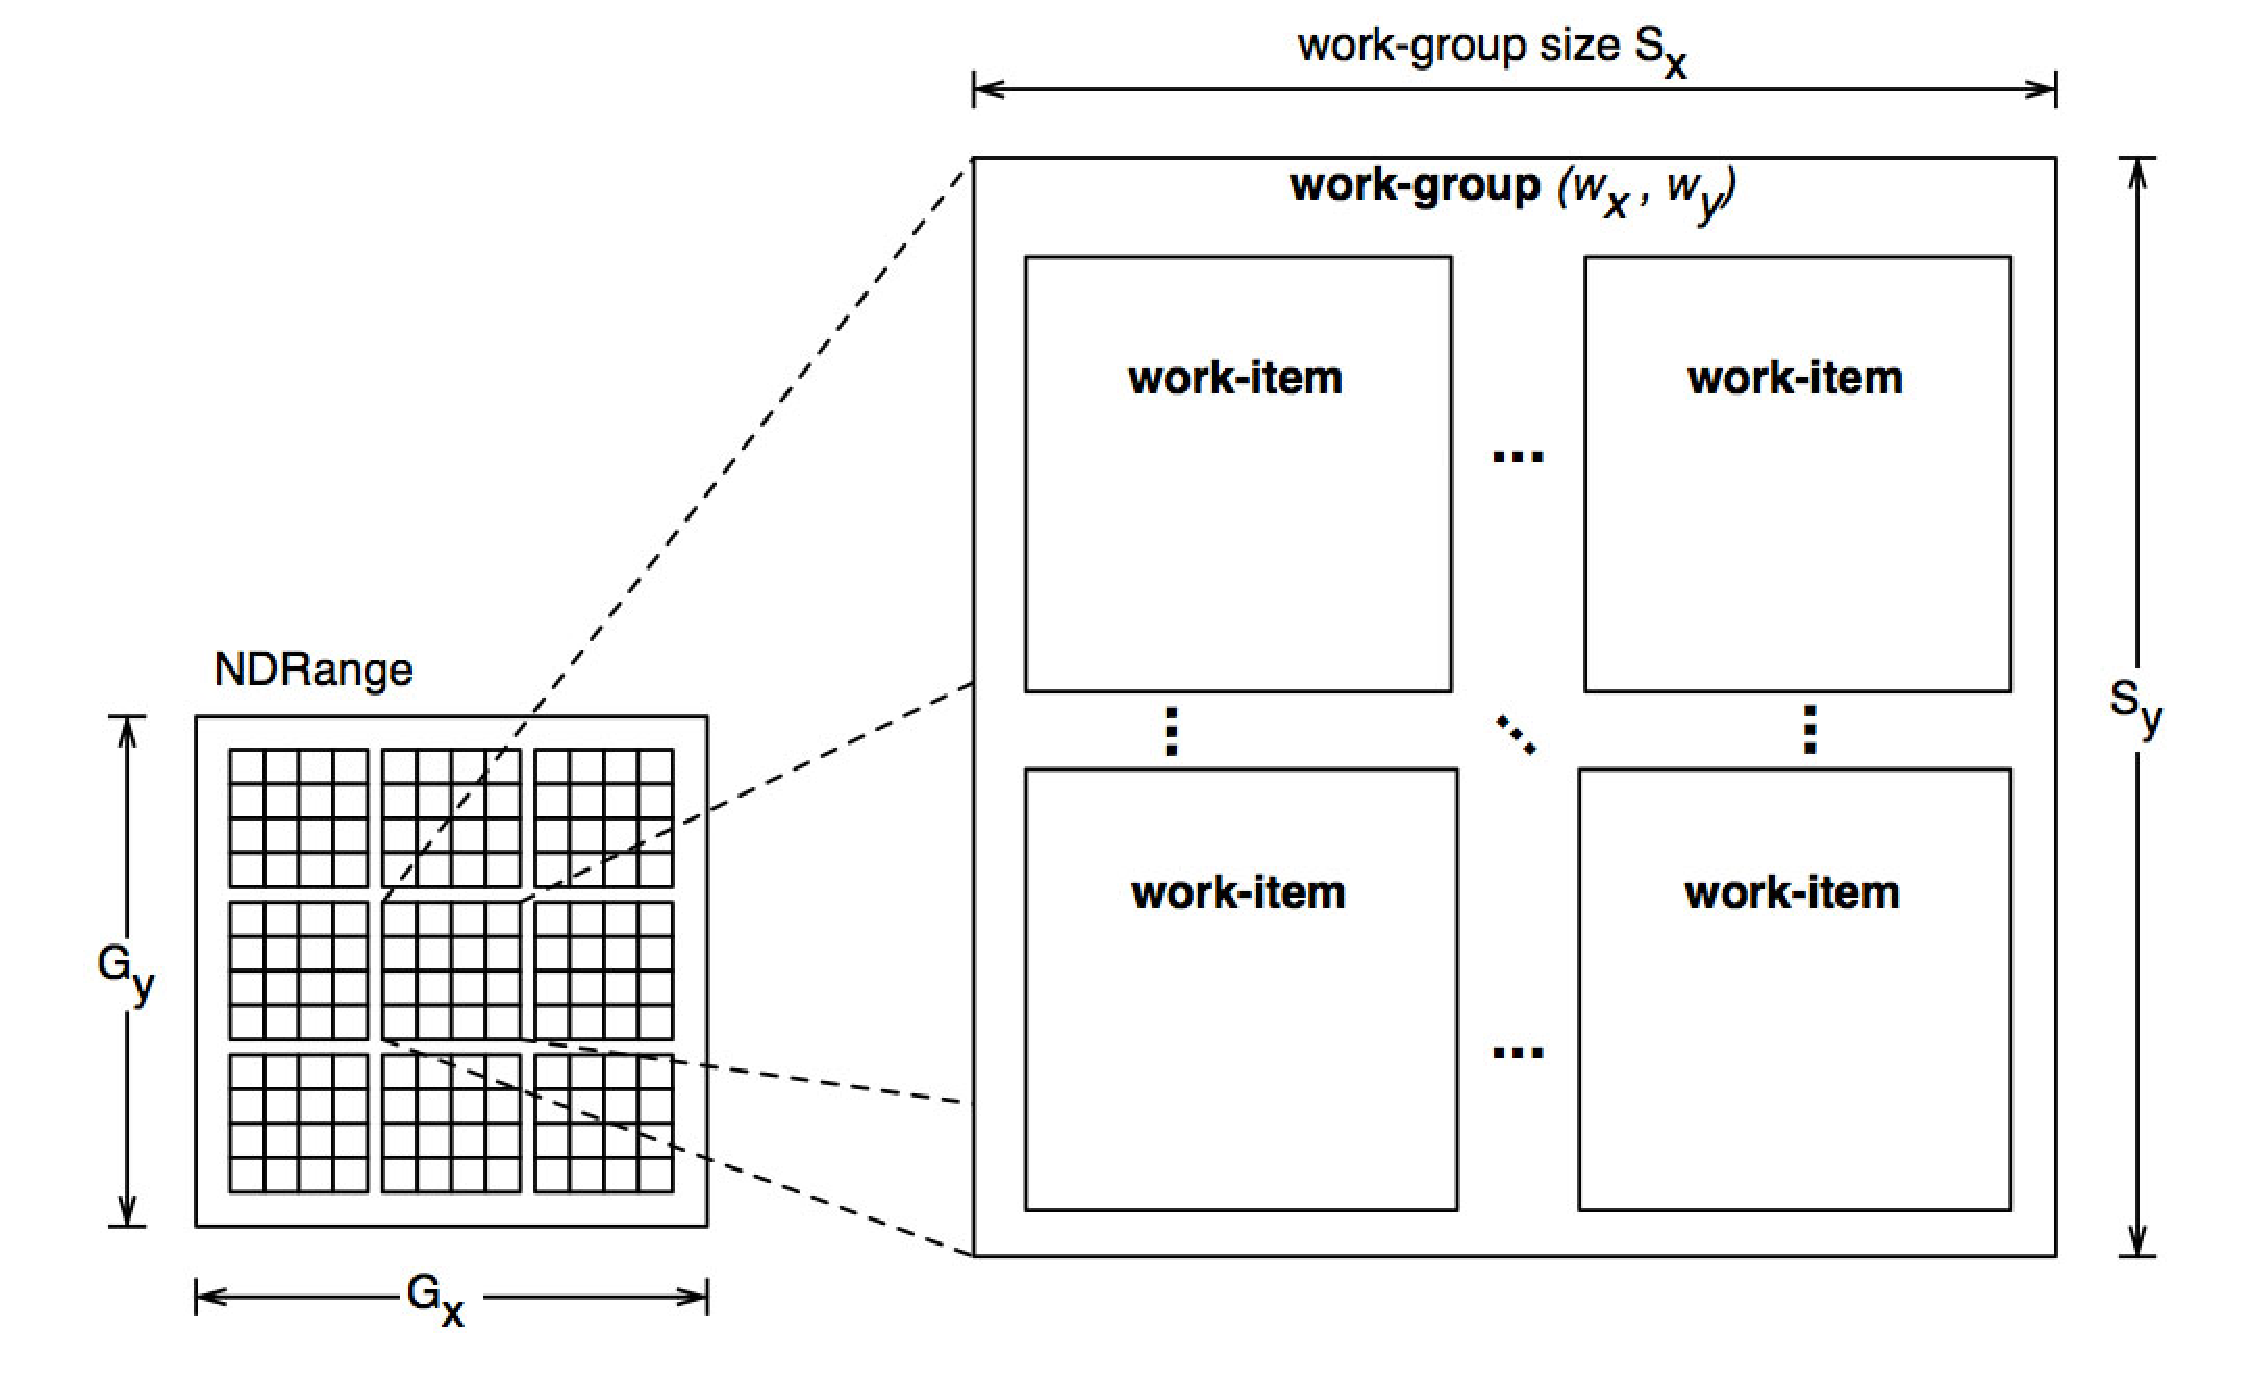
\includegraphics[width=8cm, height=4cm]{./eps/index-space.eps}
 \caption{Work-items mapped over a two-dimensional NDRange. As you can see, work-items can be organized in Work-Groups and every work-item has both a global and a local ID inside its work-group.}
 \label{fig:indexSpace}
\end{figurehere}

\begin{CLCode}
For example, to execute a kernel the host must call the \textbf{clEnqueueNDRangeKernel()} function. As you can see from the function name, kernels are not simply 'executed' but they must be added to a specific command-queue that will later be launched.
\end{CLCode}

\subsubsection{Kernel Implementation} \label{sect:kernelImplementation}
Below is an example of a simple kernel that calculates the square of the input NDRange:

{\footnotesize\begin{verbatim}
__kernel void myKernel(__global int* input,
                       __global int* output)
{
    int workID = get_global_id(0);
    output[workID] = input[workID] * input[workID];
}\end{verbatim}}

As you can see, a kernel is nothing different from a normal C/C++ function. The interesting thing of a kernel, is that it executes over \emph{each element} of the input memory object, even if no iteration is specified. This is due to the fact that when a kernel is dispatched for execution, it automatically creates multiple ``copies'' of the function (the work-item), each one with its own \textbf{workID} that maps directly to the NDRange and that will execute on a different Processing Element. Each work-item has both a \textbf{global environment} shared with all other work-items and its own \textbf{local environment} that can be accessed using the specific function that the OpenCL API offers:\\

\begin{tablehere}
{\footnotesize
\begin{tabular}{|p{3,5cm}|p{3,5cm}|}\hline
\textbf{get\_work\_dim} & Number of dimensions in use\\ \hline
\textbf{get\_global\_size} & Number of global work items\\ \hline
\textbf{get\_global\_id} & Global work item ID value\\ \hline
\textbf{get\_local\_size} & Number of local work items\\ \hline
\textbf{get\_local\_id} & Local work item ID\\ \hline
\textbf{get\_num\_groups} & Number of work groups\\ \hline
\textbf{get\_group\_id} & Work group ID\\ \hline
\end{tabular}}
  \caption{Work-Item Built-In Functions\\}
	\label{tab:workItemFunctions}
\end{tablehere}

\subsubsection{Program Context and Command-Queue} \label{sect:context}

As we alreaty mentioned, one of the host functions is to define the \textbf{context} for the application. Contexts are used by the OpenCL runtime for managing objects such as command-queues, memory, program and kernel objects and for executing kernels on one or more devices specified in the context.\\
A context basically consists in:

\begin{enumerate}
	\item a collection of \textbf{OpenCL devices} to be used
	\item a collection of the functions that will be executed on the devices (the kernels)
	\item \textbf{program objects}, that are simply the source files and executables that implements the kernels
	\item \textbf{memory objects}: the NDRange objects to be elaborated
\end{enumerate}

After the context has been created, the host initialize a structure called \textbf{command queue} that is used to schedule and dispatch commands to the devices within the context. The command structure is very simple and the commands that the host may issue fall only into three categories:

\begin{enumerate}
	\item \textbf{Kernel execution commands}: Execute a kernel on a Processing Elements of a specific device.
	\item \textbf{Memory commands}: Transfer data to, from, or between memory objects, or map and unmap
memory objects from the host address space.
	\item	\textbf{Synchronization commands}: Used to specify the order of execution of commands and to synchronize the kernels.
\end{enumerate}

\begin{CLCode}
Context and Command Queues are created by simply calling the \textbf{clCreateContext()} and \textbf{clCreateCommandQueue() 
} functions in the host.
\end{CLCode}


\subsubsection{The Memory} \label{sect:memory}

There are four types of memory regions in OpenCL: \textbf{Global Memory}, \textbf{Constant Memory}, \textbf{Local Memory} and \textbf{Private Memory}.

\begin{itemize}
	\item Global memory grants read/write privileges to \textbf{all} the work-items in every work-group. Basically, every work-item (\emph{that are part of the same context}) can access it.
	\item Constant memory is only used to store constants. Only the host has write privileges over it, while kernels can only read from it.
	\item Local memory is shared among all the work-items that form a group. The host has no access to this memory area.
	\item Private memory is allocated directly by the work-item and can be used only by itself. The host has no access to this part of memory.
\end{itemize}

Since computation is carried on parallely, one of the major issues about memory is \textbf{consistency}. OpenCL uses a relaxed consistency memory model: the state of memory visible to a work-item is not guaranteed to be consistent across the collection of work-items at all times. \textbf{Table \ref{tab:memconsistency}} summarizes memory consistency for the various regions of memory available.\\

\begin{tablehere}
{\footnotesize
\begin{tabular}{|p{2cm}|p{5,5cm}|} \hline
\textbf{Memory} & \textbf{Consistency}\\ \hline
Private & memory is not shared, read/write consistency is always guaranteed\\ \hline
Local & consistency is guaranteed between work-items of the same work-group\\ \hline
Global & consistency is guaranteed between work-items of the same work-group, but not between multiple work-groups in the case they are assigned to execute the same kernel\\ \hline
\end{tabular}}
\caption{Memory consistency\\}
\label{tab:memconsistency}
\end{tablehere}
%\vfill
%\columnbreak
In OpenCL computation is performed over \textbf{memory objects}. There are two distinct memory objects: \textbf{buffers} and \textbf{images}.

\begin{itemize}
	\item Buffers are used to store a one-dimensional collection of elements (like an array), and those elements can be scalar values (int, float, etc.), vectors or user defined structures.
	Buffers are stored sequentially and \emph{can be accessed using pointers}; elements of a buffer are stored in memory in the \emph{same format} as they are used by kernels (i.e. if the kernel works on single integers, these elements are stored in memory as integers, this is not true for image objects)
	\item Images are used to store bi- or three-dimensional structures and their elements can only be selected from a list of predefined image formats (i.e. you cannot simply declare int or floats in an image object). Differently from buffers, elements of images \emph{cannot be accessed directly with a pointer} and they are \emph{always stored in memory as 4-dimensinal vectors} (since graphic shaders work on RGB and Alpha components of the pixels of an image)
\end{itemize}

\begin{CLCode}
In OpenCL memory objects are stored into \textbf{cl\_mem} structs, that can be easily initializated with the \textbf{clCreateBuffer()} and \textbf{clCreateImage()} functions.\\
Image format availables may vary from one graphic adapter to another, a list of supported image formats can be obtained using the \textbf{clGetSupportedImageFormats()} query.
\end{CLCode}



%-----------------------------------------------------------------------------
\vfill
\columnbreak
\subsection{Device Fission Introduction}

Device Fission is an extension of the OpenCL specification (fully defined in OpenCL 1.2, although it was already available in OpenCL 1.1 as well as an optional extension) that adds a whole new level of control over parallel computation and hardware management.\\
As the term 'fission' implies (dividing or splitting something into two or more parts), device fission allows the sub-dividing of a device into one or more virtual sub-devices. This practice, when used carefully, can provide a huge performance boost, especially when executing parallel code on the CPU instead of the GPU \cite{intel:12:DeviceFission} (At present day device fission is suported only on CPUs and not on GPUs \cite{gaster:11:DeviceFission})
Implementing applications that use device fission \emph{does} require some knowledge of the underlying target hardware and, if not used properly, it can lead to worst performances and it may impact code portability.

\subsubsection{Device Fission as a better way to manage Embedded Systems}
Device fissioning can be very useful in embedded environments and, in general, in any situation where the system resources are limited:

\begin{itemize}
	\item Device fission allows to use only a \emph{portion} of a device, this means that the OpenCL runtime will not take the entire device for itself and other non-OpenCL application can work on it at the same time.\\ It can also help to reduce power consumption since high-task parallelism at low core frequencies can give better power perfomaces \cite{leskela:mobileGPGPU}
	\item Device fission allows to implement specialized memory sharing models that can be useful when it comes to manage the limited memory of an embedded system. (For example see the partitioning by affinity domain described in Section \ref{sect:memproximity})
	\item Since embedded systems may have limited graphic capabilities (or no graphic adapter at all), Device Fission may help to better exploit parallel computation where the only option is to use a CPU and not a GPU
\end{itemize}

\subsubsection{Sub Devices} \label{sect:DF-subdevices}
Each subdevice can have its own \textbf{program context} and \textbf{command-queue} (See Section \ref{sect:context}), this means that each subdevice can have its own private area of memory and that kernels can be dispatched independently to one subdevice or another.\\

\begin{CLCode}
In OpenCL you can create new sub-devices using the \textbf{clCreateSubDevices()} function. The first parameter to pass is of type \textbf{cl\_device\_id} and it is the ID of the 'parent' device to be partitioned.\\ You can query for a list of available devices on the system by using the \textbf{clGetDeviceIDs()} function. Each sub-device can have a maximum number of compute units specified by the \textbf{CL\_DEVICE\_PARTITION\_MAX\_COMPUTE\_UNITS} property.
Since sub-devices are treated in the same exact way as 'normal' devices, different contexts and command-queue can be created by simply passing the ID of the subdevice to the \textbf{clCreateContext()} and \textbf{clCreateCommandQueue()} functions .
\label{Code:DevicePartitioning}
\end{CLCode}

There are three main way to partition a device: \textbf{equally}, \textbf{by counts} and \textbf{by affinity domain}:

\begin{itemize}
	\item partitioning a device \textbf{equally} means that the application will try to split the device into as many sub-devices as possible, each containting a number of Compute Units specified by the programmer. If that number does not divide evenly into the maximum available compute units, the remaining are not used.
	\item \textbf{by counts} means that the device is not divided automatically (and equally), but accordinlgy to a list provided by the programmer (e.g. given the list (4, 8, 16) the device will be divided into three sub-devices containing respectively 4, 8 and 16 CUs)
	\item partitioning by \textbf{affinity domain} is an automatic process that will create sub-devices composed of CUs that share similar levels of cache-hierarchy (specified by the programmer, e.g. L1, L2, L3 caches or NUMA nodes). This can be very useful when micro-management of memory is useful or for system where memory is a critical factor (for example in  embedded systems)
\end{itemize}

A list of some examples on how these partitioning parameters can be used to create different configurations on the same hardware can be found in the \textbf{Appendix A}.\\
Another interesting feature that allow even more flexibility and control over the hardware is that device fission allows sub-devices to be further partitioned and therefore create a tree-like structure like the one shown in \textbf{Figure \ref{fig:subdevicestree}}:

\begin{figurehere}
 \centering
 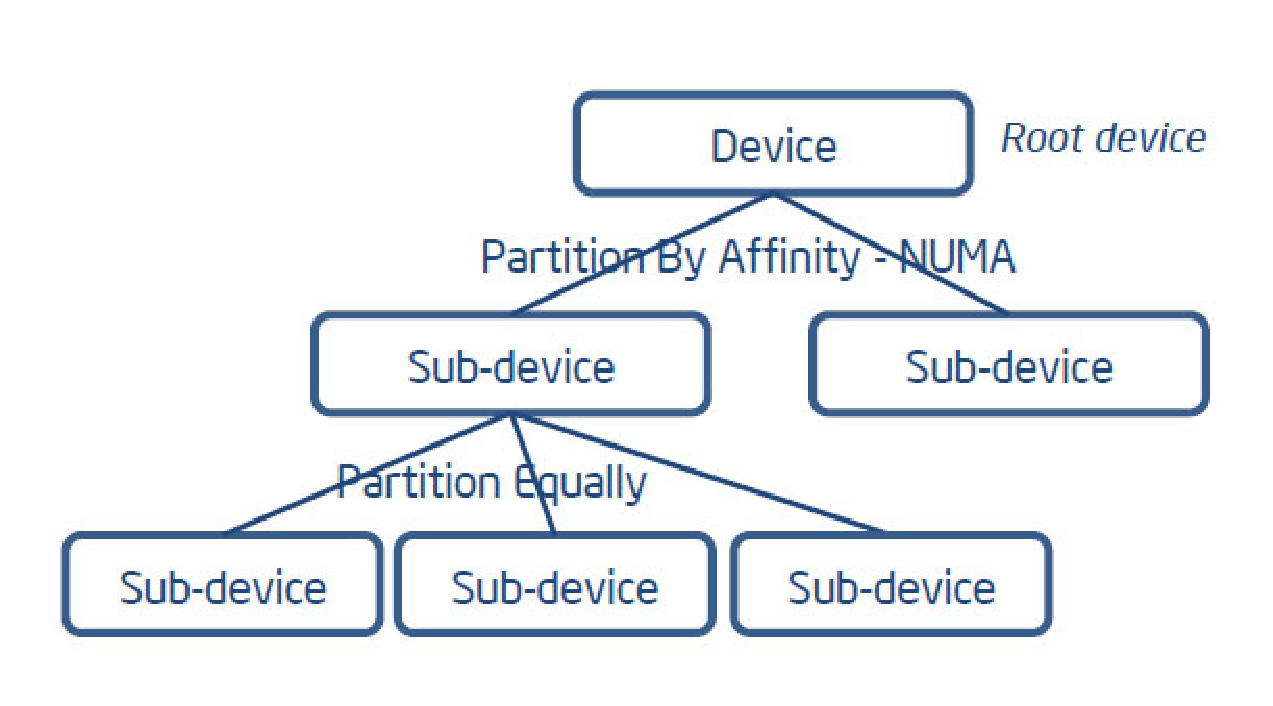
\includegraphics[width=8cm, height=4cm]{./eps/partitionTree.eps}
 \caption{Sub-devices can be further partitioned to create an hierarchy of devices. Each node of the tree can be partitioned using different partition parameters.}
 \label{fig:subdevicestree}
\end{figurehere}

\subsection{Device Fission Strategies}
Device fission can be used in several way to increase performance of OpenCL applications and to manage the (limited) resources of a system in a more efficient way. There are several standard approaches in which device fission can make the difference if used correctly and in the next sections we'll present some examples.

\subsubsection{High-Priority dedicated sub-device} \label{sect:highPriority}
\begin{figurehere}
 \centering
 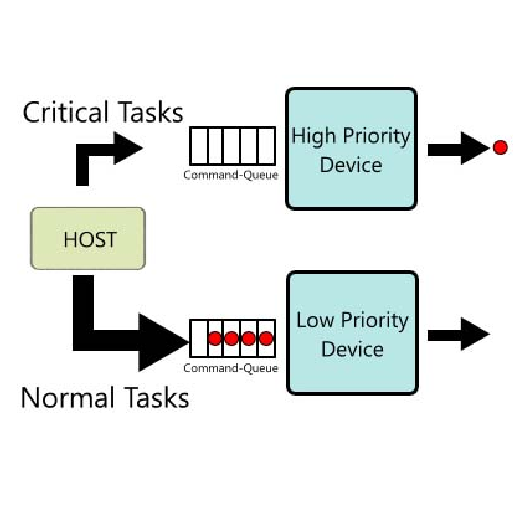
\includegraphics[width=6cm, height=6cm]{./eps/HighPriority.eps}
 \caption{Scenario 1: a sub device is created to compute high-priority tasks}
 \label{fig:highPriority}
\end{figurehere}

In this scenario, a sub-device is created to deal with critical tasks, while the remaining Compute Units of the device will be used for standard computation. Low priority tasks will be dispatched to the low priority queue, in this way the high priority device will will always have its command queue free and will be able to execute its tasks as soon as they are issued.
This configuration can be simply achieved by partitioning the device \textit{by counts}, reserving a few cores (1 or 2) for high-priority computation and leaving the rest for normal computation.\\
The following code demostrates how to partition the device properly, the full code for this scenario can be found in \textbf{Appendix \ref{Appendix:B}}.


{\footnotesize\begin{verbatim}

// Get Device ID from platform [0]
// a list of available platforms can be obtained
// using clGetPlatformIDs() function

clGetDeviceIDs( platforms[0], CL_DEVICE_TYPE_CPU,
                1, &device_id, NULL);
								
// Create two sub-devices, the parameters for the
// partitioning are storend into a 
// cl_device_partition_property array

cl_device_partition_property param[5];
param[0] = CL_DEVICE_PARTITION_BY_COUNTS;
param[1] = 2;   // 1st device: 2 compute units
param[2] = 4; 	// 2nd device: 4 compute units
param[3] = CL_DEVICE_PARTITION_BY_COUNTS_LIST_END;
param[4] = 0; //end of list

//now we can create the sub-devices
cl_device_id output_IDs[2]; 
clCreateSubDevices(device_id, param, 2,
                   output_IDs, NULL);
									
//our `High Priority' device:
cl_device_id *hpDevice = &output_IDs[0];  
//our `normal' device:    
cl_device_id *normalDevice = &output_IDs[1]; 

\end{verbatim}}

\subsubsection*{Test Results}
We partitioned a CPU device with 4 cores in total and created two sub-devices, one with 3 Compute Units (the low-priority one) and one with just one Compute Unit (the high-priority one). Then we tried to dispatch different sets of kernels marked 'normal' and 'critical'. First we dispatched all of them only to the low-priority device, and the result was that the tasks were completed in the same exact order they were dispatched, so the critical tasks had to wait for other tasks to finish. Then we routed the high priority tasks to the dedicated subdevice, with the result that those tasks were completed as soon as they were dispatched.\\
In another test we decided to block the low-priority subdevice by letting it execute an infinite while loop, the result was that the normal tasks were not able to continue their execution, but the the critical ones were still executed normally as soon as they were dispatched since they were routed to a different device.


\subsubsection{Memory Proximity} \label{sect:memproximity}

\begin{figurehere}
 \centering
 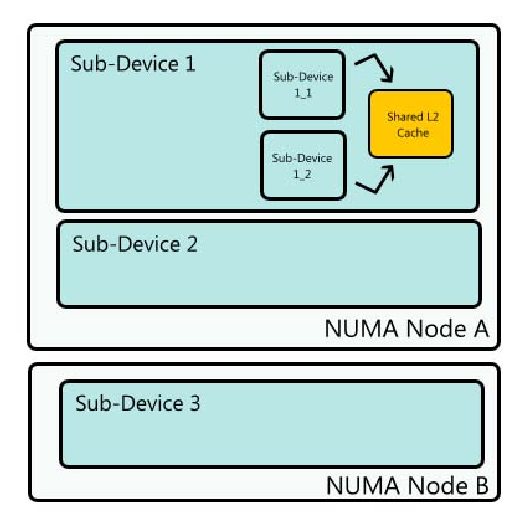
\includegraphics[width=6cm, height=6cm]{./eps/MemoryProximity.eps}
 \caption{The main device is partitioned into 2 subdevices that have Compute Units that share the same NUMA node. Subdevice 1 is further partitioned to obtain two devices that shares the same L2 Cache.}
 \label{fig:MemoryProximity}
\end{figurehere}

If the work-items of the application share high amounts of data, it can be useful to create sub-devices that share the same cache or are physically placed on the same NUMA node to increase performance.
Without device fission, there is no guarantee that the work items will have these characteristics.
This kind of partitioning can be achieved using the \textit{partition by affinity model}, specifying which level of memory needs to be shared.\\
Obviously, this kind of partition is highly hardware-dependent, and it is not guaranteed that a particular partitioning scheme will work on different platforms. To maintain portability the host should check which partition models are available on that specific device and decide at runtime how to subdivide it. 

\begin{CLCode}
The memory domains available on a particular device can be obtained by a simple query with the \textbf{clGetDeviceInfo()} passing \textbf{CL\_DEVICE\_PARTITION\_PROPERTIES} and \textbf{CL\_DEVICE\_PARTITION\_AFFINITY\_DOMAIN} as parameters.
\label{Code:MemoryDomains}
\end{CLCode}

The following example creates a partitioning model like the one shown in \textbf{Figure \ref{fig:MemoryProximity}}

{\footnotesize\begin{verbatim}
clGetDeviceIDs( platforms[0], CL_DEVICE_TYPE_CPU,
                1, &device_id, NULL);

// First partitioning
cl_device_partition_property params[3];
params[0] = CL_DEVICE_PARTITION_BT_AFFINITY_DOMAIN;
params[1] = CL_DEVICE_AFFINITY_DOMAIN_NUMA; 
params[2] = 0; // End of list

// Create the sub-devices:
cl_device_id subdevices_IDs[2];
clCreateSubDevices(device_id, params, 2,
                   subdevices_IDs, NULL);
									
// We devide the first subdevice into 2 further
// subdevices
cl_device_partition_property params[3];
params[0] = CL_DEVICE_PARTITION_BY_AFFINITY_DOMAIN;
params[1] = CL_DEVICE_AFFINITY_DOMAIN_L2_CACHE; 
params[2] = 0; // End of list

cl_device_id subsubdevices_IDs[2];
clCreateSubDevices(subdevices_IDs[0], params, 2,
                   subsubdevices_IDs, NULL);


\end{verbatim}}

The case study in Section \ref{sect:LUDeviceFission} contains an example on how partition by affinity is used to exploit temporal and spatial cache locality.

\vfill
\columnbreak

\subsubsection{Warm Cores Exploitation}

\begin{figurehere}
 \centering
 \includegraphics[width=7cm, height=10cm]{./eps/WarmCores.eps}
 \caption{Without device fission there is no real control on which cores will be used, and tasks may be dispatched to 'cold' cores. With device fission we can redirect tasks to a specific (small) subdevice and exploit 'warm' cores.}
 \label{fig:WarmCores}
\end{figurehere}

Without device fission, when a new command is submitted to the command-queue it may happen that it will be dispatched for execution to a 'cold' core. 'Cold' cores are those that have cache memory filled with data that is not relevant to the current OpenCL program or task. With device fission we can force to use already 'warmed up' cores to minimize latency time.
This scenario adapts well for short-running programs, where the overhead of `warming' the core is relevant. For long-running programs, using device fission in this way may have very little effect or even degrade performance.
This approach can also be used for thermal management purposes, as it can have effect on which area of the CPU will heat more.\\
The implementation of this kind of behavior is similar to the one described in Section \ref{sect:highPriority}: we can divide the device by \textit{counts}, reserving a 'warm' area over which we will dispatch fast and short tasks.

\subsubsection{Flowgraph and Pipeline Computation} \label{sect:pipelineScenario}

\begin{figurehere}
 \centering
 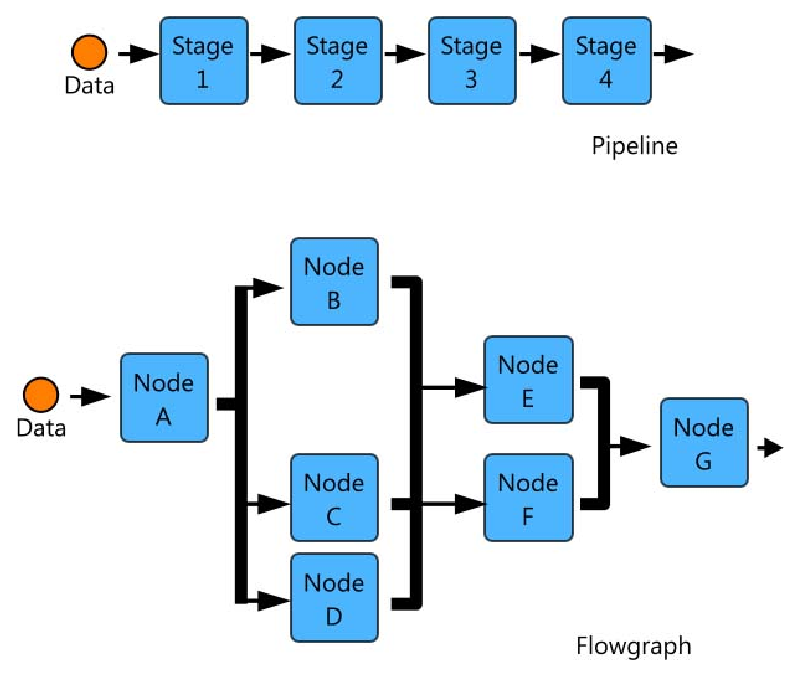
\includegraphics[width=8cm, height=7cm]{./eps/flow.eps}
 \caption{Device partitioning allows to create 'virtual' pipelines}
 \label{fig:flow}
\end{figurehere}

Since device fission gives total control over task dispatching, we can use it to create complex structures like the one shown in \textbf{Figure \ref{fig:flow}}. This technique allows to create high-specialized virtual devices (like virtual hardware) for carrying out specific tasks and a good synchronization from the host must be provided. 

\subsubsection{Maximize Throughput}
This scenario applies when data sharing is very limited or completely absent, and the only important thing is to maintain high levels of throughput. To achieve this, a job must have \textit{all the resources} available for itself (i.e. all the on-chip caches), and no other jobs may interfere, therefore we must create \emph{one and only one} device for each NUMA node, so devices will never try to access the caches of other devices.\\
To create this kind of partitioning Partition By Affinity must be used to fission the device into N sub-devices, where N is the number of NUMA node available.

\vfill
\columnbreak







